\documentclass[tikz,border=10pt]{standalone}
\usepackage{amsmath}
\usepackage{amssymb}
\definecolor{mantis}{RGB}{0, 105, 62}
\begin{document}
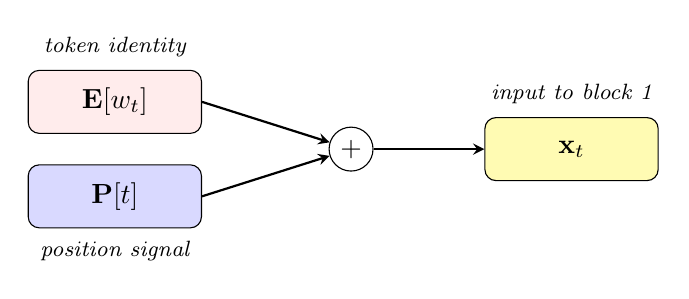
\begin{tikzpicture}[>=stealth]
    \node[draw, rounded corners, fill=pink!30, minimum width=2.2cm, minimum height=0.8cm] (emb) at (0,0.6) {$\mathbf{E}[w_t]$};
    \node[draw, rounded corners, fill=blue!15, minimum width=2.2cm, minimum height=0.8cm] (pos) at (0,-0.6) {$\mathbf{P}[t]$};
    \node[draw, circle, fill=white, inner sep=2pt] (plus) at (3,0) {$+$};
    \node[draw, rounded corners, fill=yellow!30, minimum width=2.2cm, minimum height=0.8cm] (xt) at (5.8,0) {$\mathbf{x}_t$};
    \draw[->, thick] (emb.east) -- (plus);
    \draw[->, thick] (pos.east) -- (plus);
    \draw[->, thick] (plus) -- (xt);
    \node[font=\footnotesize\itshape] at (0,1.3) {token identity};
    \node[font=\footnotesize\itshape] at (0,-1.3) {position signal};
    \node[font=\footnotesize\itshape] at (5.8,0.7) {input to block 1};
\end{tikzpicture}
\end{document}
